\documentclass{article}

\usepackage[utf8]{inputenc}

\usepackage{makecell}
\usepackage{tikz}
\usetikzlibrary{automata}

\begin{document}

\tikzset{
    state/.style={
        rectangle,
        rounded corners, 
        draw=black, very thick,
        text width = 3cm,
        minimum height = 1.5cm,
        inner sep=2pt,
        text centered,
    },
}

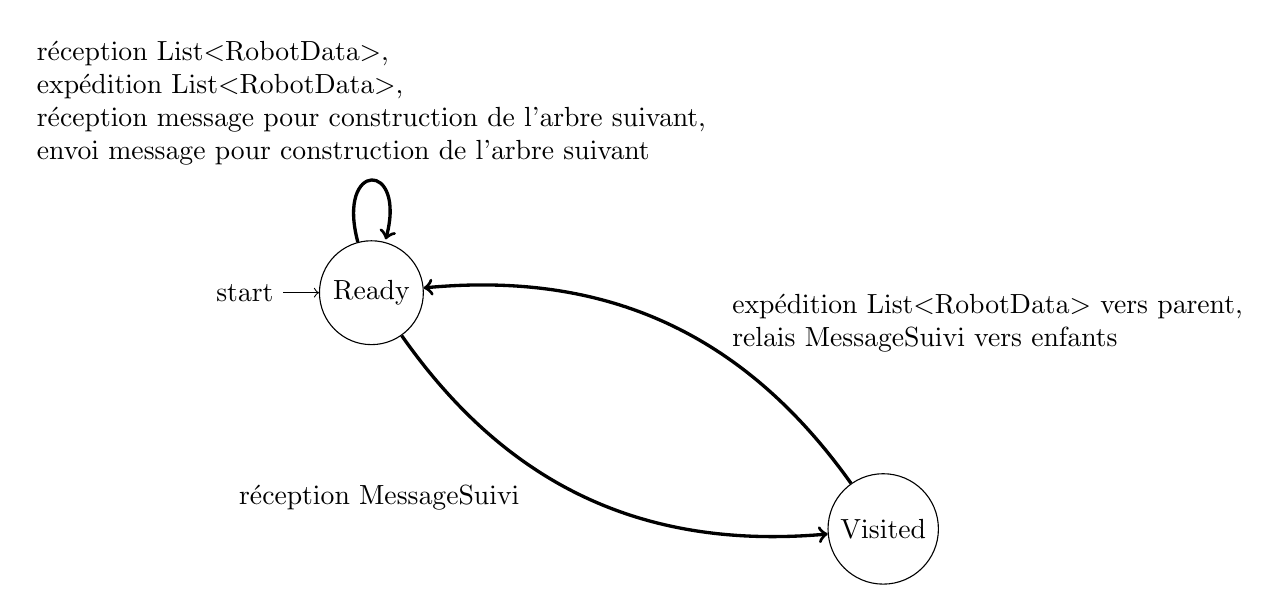
\begin{tikzpicture}

\node[state, 
      initial] 
(q1) { Ready };

\node[state,   
      right of = q1,
      yshift = -3cm, 
      node distance = 6.5cm,
      anchor = center] 
(q2) { Visited };

\draw[very thick,->] 
    (q1) 
    edge[bend right, below] 
    node[left, 
         xshift = -2em] 
    { réception MessageSuivi } 
    (q2)
    %
    (q2) 
    edge[bend right, above] 
    node[right, 
         xshift = 2em]
    {\makecell[l]{
        expédition List$<$RobotData$>$ vers parent, \\
        relais MessageSuivi vers enfants}} 
    (q1)
     %
    (q1) 
    edge[loop above] 
    node
    {\makecell[l]{
        réception List$<$RobotData$>$, \\
        expédition List$<$RobotData$>$, \\
        réception message pour construction de l'arbre suivant, \\
        envoi message pour construction de l'arbre suivant} } 
    (q1);
\end{tikzpicture}

\end{document}